\section{Développement}

\subsection{Les métadonnées}

\begin{frame}
	\frametitle{\insertsubsectionhead}
	\pause
	\begin{block}{Des métadonnées en communs}
		\begin{itemize}
			\pause
		\item le \textit{MAGIC}
			\pause
		\item Version
			\pause
		\item Algorithme de chiffrement et de hashage
			\pause
		\item Sel
			\pause
		\item nombre d'itérations pour PKCS5v2
			\pause
		\item clé maître chiffrée
		\end{itemize}
	\end{block}
\end{frame}

\begin{frame}
	\frametitle{\insertsubsectionhead - \textbf{FreeBSD}}
	\begin{figure}
		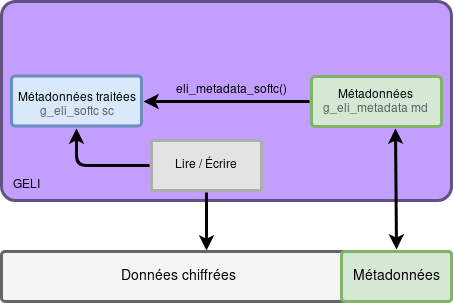
\includegraphics[width=.8\textwidth]{developpement/utilisation_metadonnee}
		\caption{Utilisation des métadonnées dans FreeBSD}
	\end{figure}
\end{frame}

\begin{frame}
	\frametitle{\insertsubsectionhead - Utilisation dans le code}
	\begin{figure}
		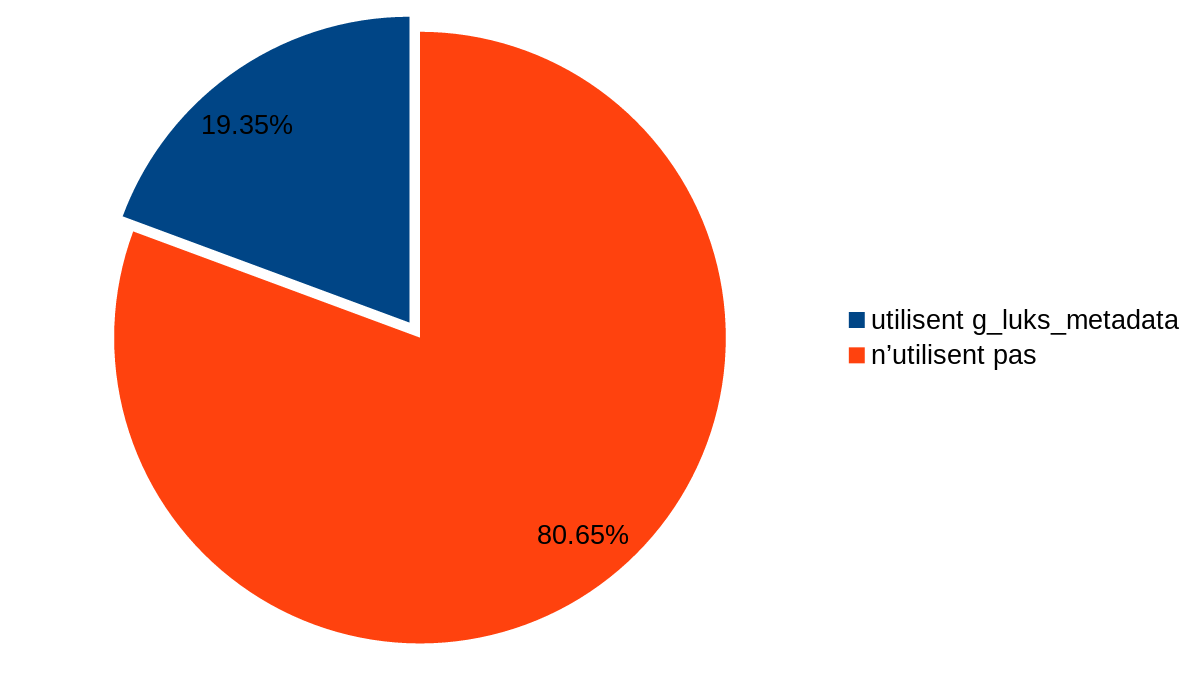
\includegraphics[width=.8\textwidth]{developpement/fonctions_g_luks_metadata}
		\caption{Utilisation de la structure g\_luks\_metadata}
	\end{figure}
\end{frame}
\begin{frame}
	\frametitle{\insertsubsectionhead - Utilisation dans le code}
	\begin{figure}
		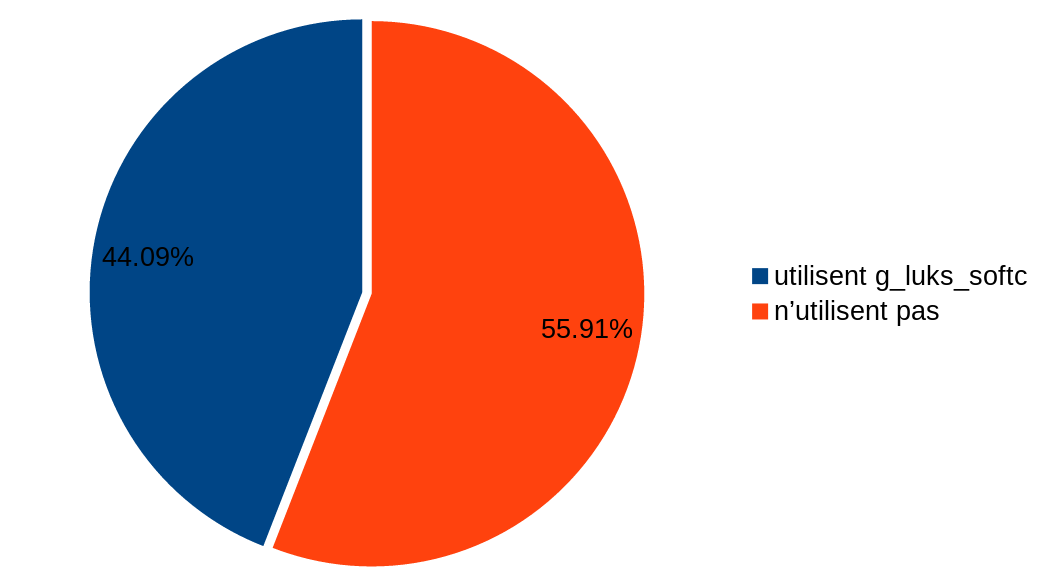
\includegraphics[width=.8\textwidth]{developpement/fonctions_g_luks_softc}
		\caption{Utilisation de la structure g\_luks\_softc}
	\end{figure}
\end{frame}

\begin{frame}
	\frametitle{\insertsubsectionhead - Transformation des métadonnées}
	\begin{figure}
		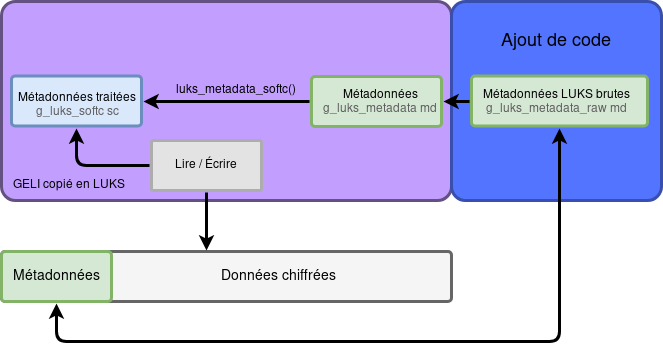
\includegraphics[width=\textwidth]{developpement/utilisation_metadonnee_luks}
		\caption{Introduction d'un structure intermédiaire}
	\end{figure}
\end{frame}

\subsection{Déchiffrement de la clé}

\begin{frame}
	\frametitle{\insertsubsectionhead}
\end{frame}	
